Sikteerin tärkein uudistus on käyttäjän tunnistamiseen käytettävien tietojen (salasana) siirtäminen pois sen omasta SQL-tietokannasta. Sikteerin omaan tietokantaan tallennetaan jatkossakin niiden käyttäjien tiedot, joilla on pääsy järjestelmään, koska käyttäjällä on vain Sikteeriin liittyviä attribuutteja, joita ei haluta tallentaa käyttäjähallintaan. Näin Sikteerin omaa tietokantaa käytetään pääsynvalvonnassa: tunnistamisen jälkeen Sikteeriin pääsevät vain käyttäjät, joiden käyttäjätunnusta vastaava rivi on kirjattu tietokantaan.

Käyttäjätunnus yksilöi käyttäjän Kapsin järjestelmissä, joten sitä voidaan käyttää avaimena Sikteerin ja tunnistautumispalvelun välillä. Tunnistamisen jälkeen tunnistautumispalvelusta tuleva käyttäjän data sisältää tiedon myös käyttäjätunnuksesta, jota käytetään käyttäjän yksilöivänä tunnisteena, kun käyttäjän pääsyoikeus tarkistetaan Sikteerin tietokannasta.

Käytännön tasolla uutta keskitettyä tunnistautumispalvelua käytettäessä väliohjelmakerroksessa tunnistautumista tekevän väliohjelman toimintaa muutetaan. Nykyisessä toteutuksessa väliohjelma vertaa käyttäjän syöttämää tunnusta ja salasanaa paikallisesta tietokannasta löytyviin. Uudistuksen jälkeen käyttäjätunnus selvitetään ulkoisen palvelun avulla, jonka jälkeen tunnukseen liittyvät attribuutit haetaan paikallisesta kannasta. Väliohjelman muutoksen lisäksi muita muutoksia Sikteerin ohjelmakoodiin ei tarvita.

Uudistetun Sikteerin toiminta on esitetty kuvassa \ref{auth_kapsi_fi_flow}. Sikteeri ohjaa ylläpitäjän tunnistautumispalveluun, josta lähetetään onnistuneen tunnistautumisen jälkeen valtuutusavain Sikteerille. Valtuutusavaimella Sikteerin väliohjelmisto hakee käyttäjän tiedot tunnistautumispalvelusta ja etsii tietokannastaan käyttäjätunnusta vastaavan käyttäjän tiedot tarkistaakseen pääsyoikeuden. Kuvassa näkyy myös tunnistautumispalvelun rajapinnat. Ensimmäisen rajapinnan kautta käyttäjä saa tunnusta ja salasanaa vasten valtuutusavaimen omiin tietoihinsa. Toinen rajapinta palauttaa käyttäjän tiedot valtuutusavainta vastaan. Tunnistautumispalvelun toteutus käydään tarkemmin läpi seuraavassa alaluvussa.

\begin{figure}[ht]
\centering
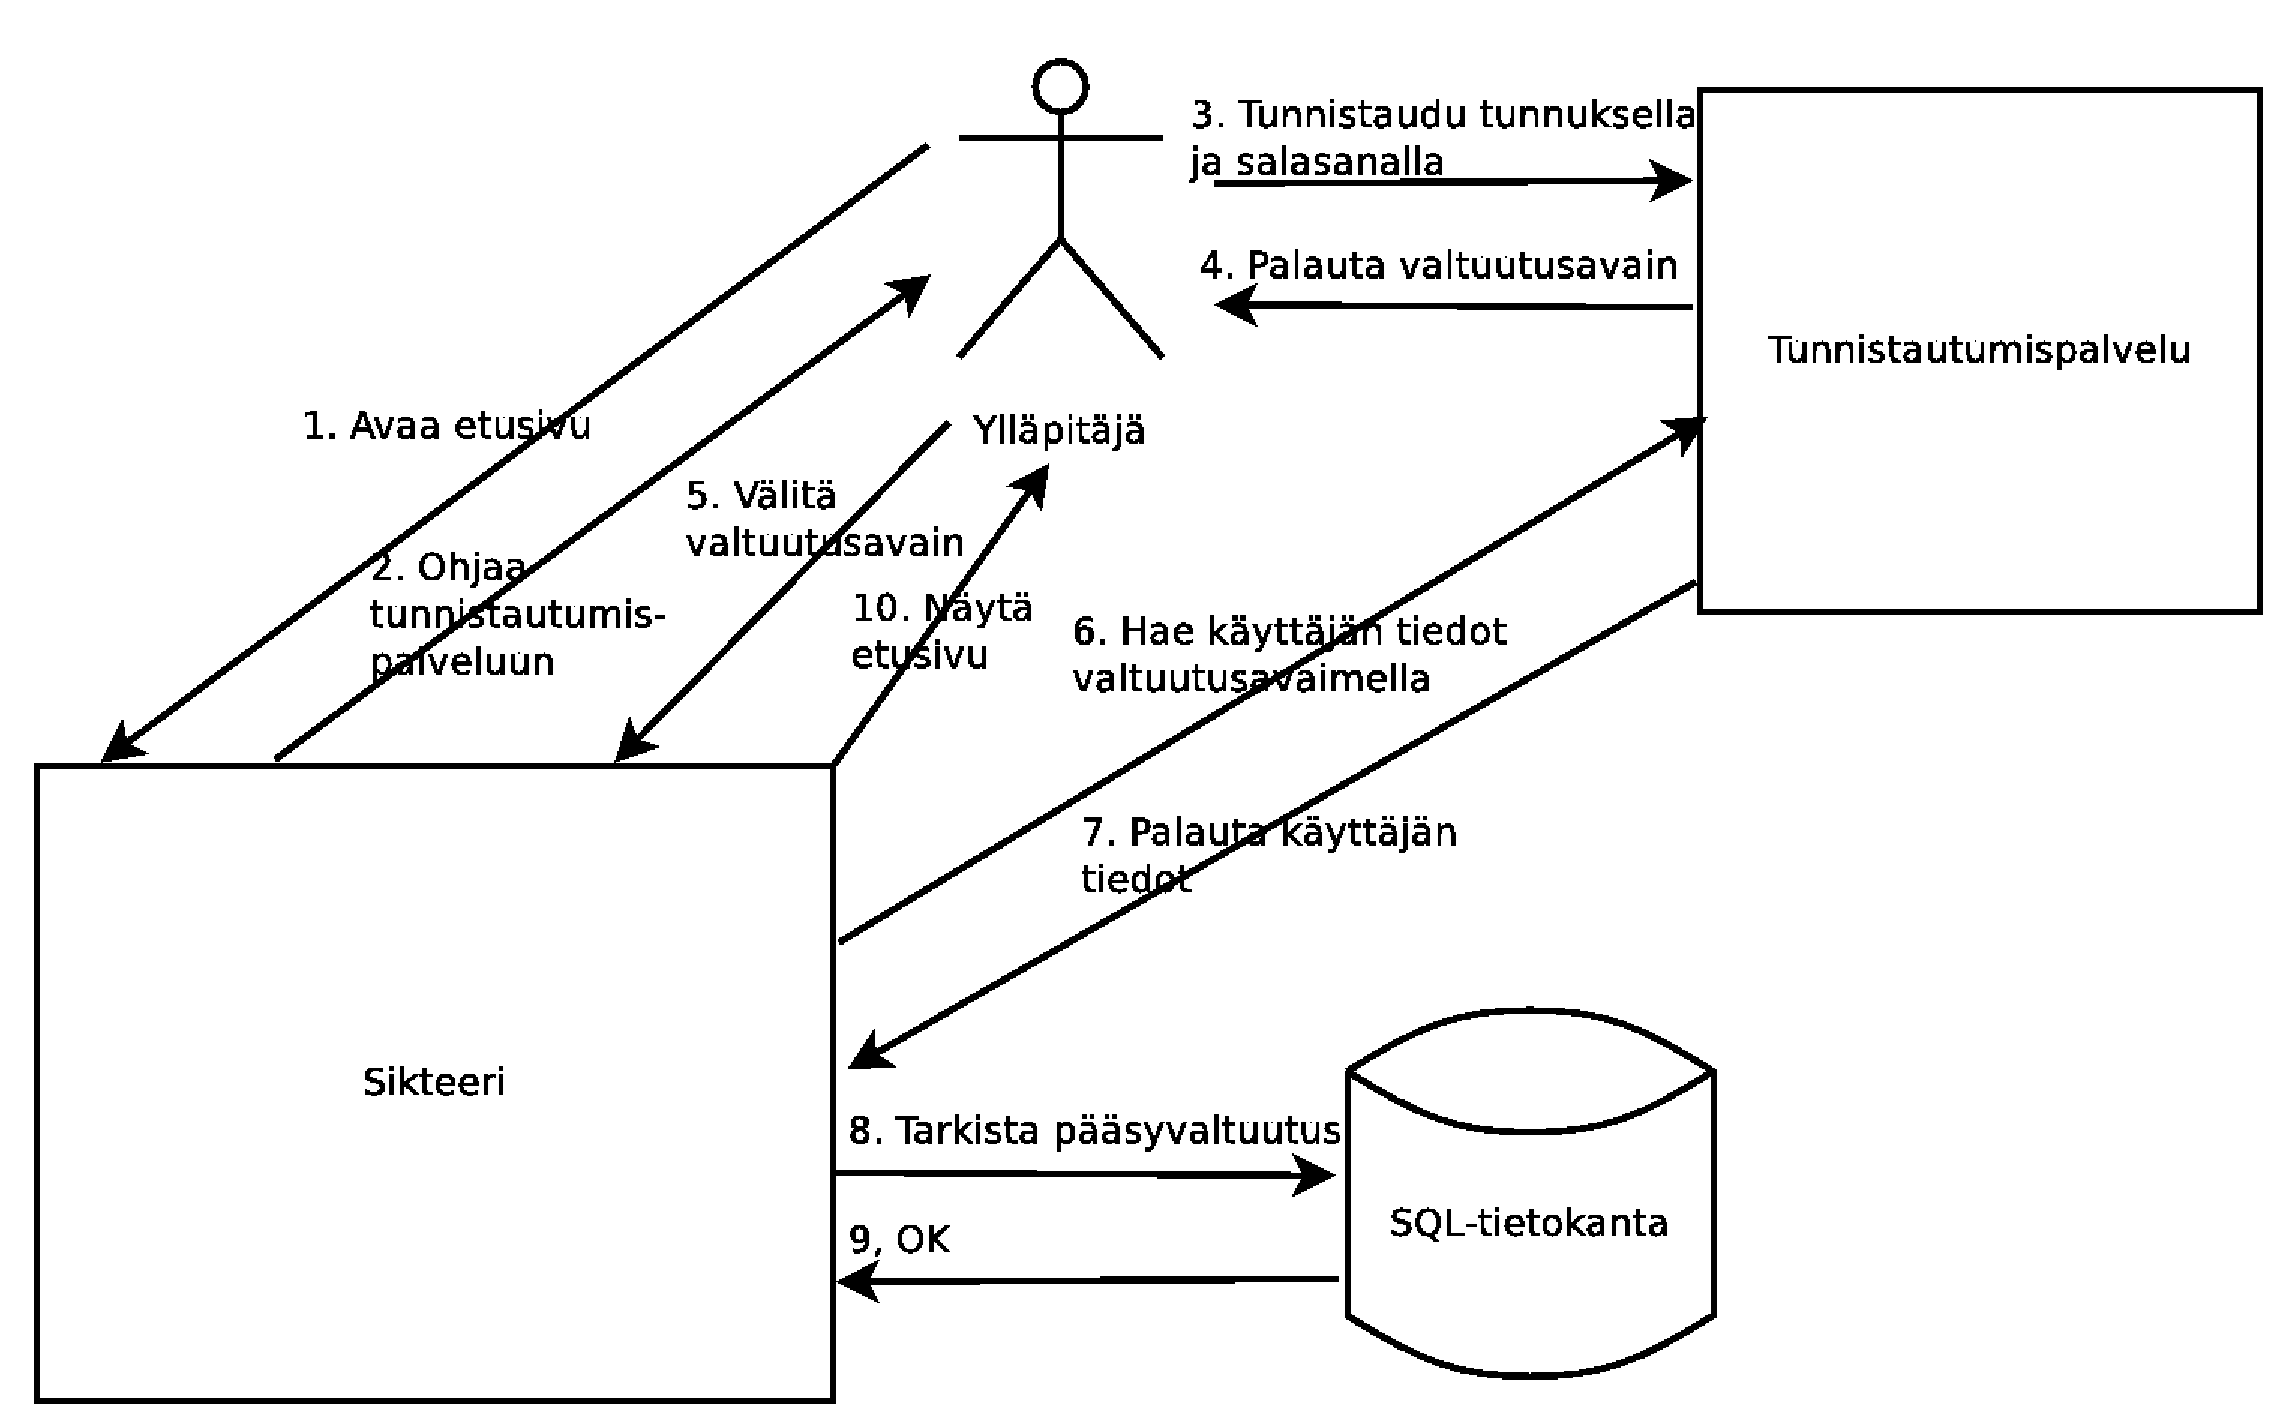
\includegraphics[width=\textwidth]{toteutus/arkkitehtuuri/auth_kapsi_fi_flow.eps}
\caption{Kontrollin kulku arkkitehtuurissa, kun ylläpitäjä alkaa käyttää Sikteeriä.}%
\label{auth_kapsi_fi_flow}
\end{figure}